\section{Computational Methods}
% TODO edit here
In our calculations, we employ a model \ce{(H2O)4} cluster that has been investigated in earlier studies by our group.\cite{10.1063/1.4991497,10.1021/acs.jpca.8b11881}
In this model, depicted in Figure~\ref{fig:water4cluster}, the monomers are arranged so that the net dipole moment is zero.
If the distance R is varied, with all other geometrical parameters held fixed, the system can be tuned from a regime (large R) that the excess electron weakly binds in the HF approximation to one (small R) at which it is not bound in the HF approximation. i.e., at which it is NVCB in nature.

\begin{figure}
    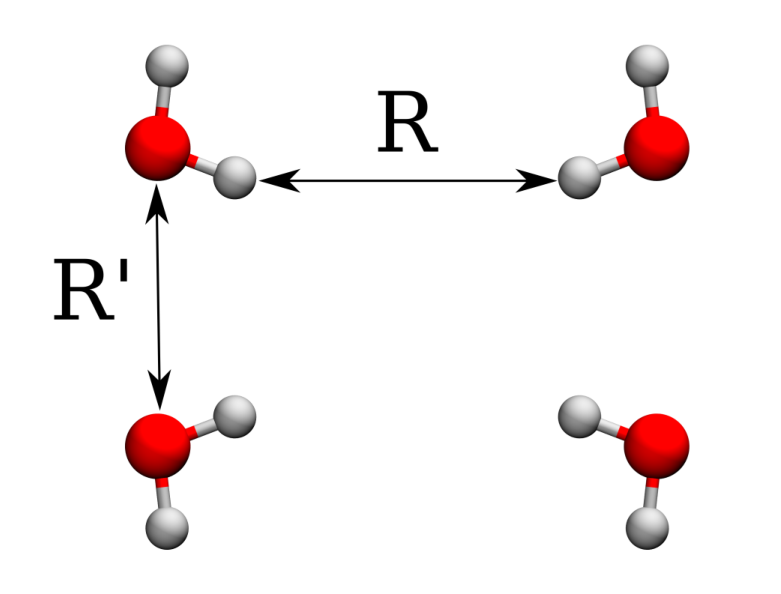
\includegraphics[width=\columnwidth,keepaspectratio]{Images/chapter3/h2o4_labeled.eps}
    \caption{\label{fig:water4cluster} The  model \ce{(H2O)4} system considered in this study. R$^{'}$ held fixed at \SI{3.46105}{\angstrom}, and R is either \SI{4}{\angstrom} or \SI{7}{\angstrom}. Image generated using VMD.\cite{10.1016/0263-78559600018-5}}
\end{figure}

\section{Methodology}
\subsection{EOM Coupled Cluster}
\label{sub:EOM}
The EOM methods considered in this study are EOM-MP2,\cite{10.1063/1.469817} EOM-CCSD,\cite{10.1016/0009-26149389023-B} EOM-CCSD(T)(a)$^*$,\cite{10.1063/1.4962910} and EOM-CCSDT,\cite{10.1063/1.1416173,10.1063/1.1378323} listed in order of increasing sophistication in terms of treatment of correlation effects. 
In the EOM-MP2 and EOM-CCSD methods, the neutral molecule is treated at the MP2 and CCSD levels, respectively, and the amplitudes from these calculations are used to perform unitary transformation of the Hamiltonian.
This "dressed" Hamiltonian is then used to carry out a 1-particle plus 2-particle-1-hole configuration interaction (CI) calculation on the anion.
In the EOM-CCSDT method, the neutral species is first treated at the CCSDT level, and the transformed Hamiltonian is used to do CI calculation on the anion that includes up to 3-particle-2-hole configurations.
The EOM-CCSD(T)(a)$^*$ method includes in an approximate manner both triple excitations in the ground state coupled cluster calculations and 3-particle-2-hole excitations in the treatment of the anion.\cite{10.1063/1.4962910}

The main basis set used for the EOM calculations reported in this study is aug-cc-pVTZ+7s7p, formed by supplementing the aug-cc-pVTZ Gaussian-type orbital (GTO) basis set\cite{10.1063/1.456153,10.1063/1.462569} with a 7s7p set of diffuse functions centered at the middle of the cluster and similar to the set from Ref.%~\onlinecite{10.1063/1.4991497}.%TODO FIX onlinecite
The exponents of the supplemental functions start at 0.023622, with each successive exponent being smaller by a factor of 3.2. 
However, as seen from Table~\ref{tab:diffusebasistuning}, the supplemental 7s7p set of diffuse functions can be truncated to 3s1p without significantly impacting the EBE as calculated at the EOM-CCSD level.
Moreover, as shown in Table~\ref{tab:corebasistuning}, expanding the main basis set (i.e., the non-supplemented portion) from aug-cc-pVTZ to aug-cc-pVQZ\cite{10.1063/1.456153,10.1063/1.462569} makes only a small impact on the EBE (~4\% at R = \SI{4}{\angstrom}) .
In contrast, reducing the main basis set to aug-cc-pVDZ\cite{10.1063/1.456153,10.1063/1.462569} leads to a ~14\% reduction in the EBE.
(These results were obtained using the EOM-MP2 method, but as seen from comparison of the results in Tables~\ref{tab:diffusebasistuning} and \ref{tab:corebasistuning}, using the aug-cc-pVTZ+3s1p basis set in both cases, the EBEs from the calculations with the EOM-CCSD and EOM-MP2 methods agree to within 0.5 meV.)
The smaller aug-cc-pVDZ+3s1p basis will be used in the EOM-CCSDT calculations, which would have been computationally prohibitive with aug-cc-pVTZ+7s7p or aug-cc-pVTZ+3s1p basis sets.
Finally, EOM-CCSD(T)(a)* calculations were carried out with aug-cc-pVTZ+3s1p3d basis sets, where the exponents of the d functions match those of the s and p functions, to assess the importance of supplemental d functions on the EBEs.
The EOM calculations utilized the frozen core approximation and were carried out using the CFOUR program.\cite{cfour,10.1063/5.0004837}%this cfour citation is ok
% checked by shiv 9/24/20 13:52
\begin{table*}
    \caption{\label{tab:diffusebasistuning}Dependence of the total energies and the EBE of the model \ce{(H2O)4} cluster at R = \SI{4}{\angstrom} on the supplemental diffuse basis functions. Results obtained using the EOM-CCSD method.}
%\begin{ruledtabular}
\begin{tabular}{l c c c}
basis set            & neutral (Ha)  & anion (Ha)    & EBE (meV)            \\
\hline
aug-cc-pVTZ      & -305.327947          & -305.331344          &   92.4            \\
aug-cc-pVTZ+1s   & -305.327953          & -305.332359          &  119.9             \\
aug-cc-pVTZ+2s   & -305.327957          & -305.334226          &  170.6              \\
aug-cc-pVTZ+3s   & -305.327958          & -305.334460          &  176.9              \\
aug-cc-pVTZ+7s   & -305.327958          & -305.334462          &  177.0              \\ \hline
aug-cc-pVTZ+7s1p & -305.327979          & -305.334604          &  180.3              \\
aug-cc-pVTZ+7s7p & -305.327987          & -305.334622          &  180.6              \\ \hline
aug-cc-pVTZ+3s1p & -305.327979          & -305.334602          &  180.2     
\end{tabular}
%%\end{ruledtabular}
\end{table*}


% checked by shiv 9/24/20 13:57
\begin{table}
    \caption{\label{tab:corebasistuning}Sensitivity of the EBE of the \ce{(H2O)4} model to the ``core'' basis set. Results obtained using the EOM-MP2 method.}
%\begin{ruledtabular}
    \begin{tabular}{lccc}
                 & Neutral (Ha)          & Anion (Ha)             & EBE (meV)                      \\ \hline
\multicolumn{4}{c}{R = \SI{4.0}{\angstrom}}                                                        \\
aug-cc-pVDZ+3s1p & -305.0371957          & -305.0428558           & 154.0                     \\
aug-cc-pVTZ+3s1p & -305.3092869          & -305.3159306           & 180.8                     \\
aug-cc-pVQZ+3s1p & -305.4008845          & -305.4078074           & 188.4                     \\ \hline
\multicolumn{4}{c}{R = \SI{7.0}{\angstrom}}                                                   \\
aug-cc-pVDZ+3s1p & -305.0383747          & -305.0432259           & 132.0                     \\
aug-cc-pVTZ+3s1p & -305.3104923          & -305.3157472           & 143.0                     \\
aug-cc-pVQZ+3s1p & -305.4021640          & -305.4075716           & 147.1                    
\end{tabular}
%\end{ruledtabular}
\end{table}

\subsection{DMC}
The DMC calculations were carried out using trial wave functions represented as products of one or more Slater determinants with a Jastrow factor with one-, two-, and three-body terms.\cite{10.1103/PhysRev.98.1479,10.1103/PhysRevB.70.235119,10.1088/1361-648X/aab9c3} 
The parameters in the Jastrow factors were optimized using variational Monte Carlo (VMC), and the resulting trial wave functions were then employed in subsequent DMC calculations.
Three types of SD trial wave functions were employed. 
These used HF orbitals, Becke-Lee-Yang-Parr (B3LYP) DFT orbitals,\cite{10.1103/PhysRevA.38.3098,10.1103/PhysRevB.37.785,10.1139/p80-159, 10.1021/j100096a001} and natural orbitals (NOs) from small restricted single plus double excitation configuration interaction (SDCI) calculations designed to bind the excess electron when it is not bound in the HF approximation.
In addition, DMC calculation were carried out using MD trial wave functions, with the determinants being determined either from the restricted SDCI procedure or from configuration interaction using a perturbative selection made iteratively (CIPSI) calculations.\cite{10.1063/1.1679199}
Details on these calculations are provided below.

To reduce the computational cost of the DMC calculations, the ccECP pseudopotentials\cite{10.1063/1.4995643,10.1063/1.5040472} were employed together with GTO basis sets that we designate as cc-pVDZ / ccECP, aug-cc-pVDZ / ccECP, aug-cc-pVDZ / ccECP+3s1p, and aug-cc-pVDZ / ccECP+7s7p. 
The "core" cc-pVDZ / ccECP\cite{10.1063/1.4995643,10.1063/1.5040472} basis set was designed for use with the ccECP pseudopotentials; the "aug" indicates that the diffuse aug functions from the aug-cc-pVDZ basis sets of Dunning and co-workers are included; and the 7s7p set of diffuse functions are those described above in the Section \ref{sub:EOM}.\cite{10.1063/1.462569}
The T-moves scheme was used to control the localization error for nonlocal pseudopotentials.\cite{10.1103/PhysRevB.74.161102}

The double-zeta rather than the larger triple-zeta basis set was used as the core basis set due to the relative insensitivity of DMC calculations to the choice of the atomic basis set. 
For most of the DMC calculations a fixed population of 16,000 walkers and time steps of 0.001, 0.003, and 0.005 a.u. were employed, with the reported results obtained by linear extrapolation to zero time step.
However, this population is much larger and the time steps much smaller than what is actually required to achieve well converged energies with minimized finite time step and fixed population errors.
% These time step and populations were chosen to mitigate the finite-time step and fixed-population errors, however these choices do not reflect a reasonable balance between computational cost and accuracy since such small time steps and large populations are not required to reasonably address these errors.  
Indeed, DMC calculations using Hartree-Fock trial wave functions, larger time steps (specifically 0.05, 0.1, and 0.2 a.u.) and a smaller population of only 1,000 walkers produce an electron binding energy within error bars of that obtained using the smaller time steps and larger populations.
Additionally, a DMC calculation with a B3LYP trial wave function with a time step of 0.05 is in agreement with the values obtained with the smaller time steps and larger populations suggesting that these parameters do not depend strongly on the choice of starting orbitals.
In light of this, the 0.05 a.u. time step and smaller walker population were employed in the DMC calculations using CIPSI trial wave functions to mitigate the additional cost associated with the MD space. 
The VMC and DMC calculations were carried out using the QMCPACK code.\cite{10.1088/1361-648X/aab9c3,10.1063/5.0004860}
The orbitals for the SD-based trial wave functions and the restricted SDCI MD wave function were both generated using GAMESS,\cite{10.1002/jcc.540141112,10.1016/B978-044451719-7/50084-6,10.1063/5.0005188} whereas the CIPSI wave functions were generated using the Quantum Package 2.0 code.\cite{10.1021/acs.jctc.9b00176} 

\subsection{Restricted CI and CIPSI-generated Trial Wave Functions for DMC Calculations}
\label{subsec:rSDCI}
The restricted SDCI procedure employed the HF wave function for the neutral molecule and a specially tailored SDCI wave function for the anion, which included all symmetry-allowed single and double excitations, with the latter restricted so that one of the electrons excited is from the orbital occupied by the excess electron in the HF wave function.
This approach, when used with a flexible basis, gives a bound anion.
NOs were generated from the SDCI wave function of the anion and were used in a SD trial wave function for subsequent DMC calculations.
In addition, the SDCI wave function itself (expanded in terms of HF orbitals) was used in MD DMC calculations on the anion for R = \SI{4}{\angstrom}. 
In this case, a threshold of 0.001 on the magnitude of coefficients in the CI expansion was used in choosing the retained determinants.
This resulted in a wave function with 1,392 Slater determinants.

By design, the restricted SDCI wave function does not allow for change of the correlation energy of the valence electrons due to the presence of the excess electron.
This possibility is allowed for in the CIPSI MD trial wave functions.
The CIPSI calculations were carried out using B3LYP orbitals rather than Hartree-Fock orbitals because the former avoids the problem of collapse onto a discretized continuum solution at R =  \SI{4}{\angstrom}.\cite{10.1103/PhysRevA.38.3098,10.1103/PhysRevB.37.785,10.1139/p80-159}
Since the CIPSI calculations have not approached the full configuration interaction limit as indicated by the second-order perturbative correction to the energy, a judicious choice of starting orbitals is required to construct a physically meaningful trial wave function.
In order to generate compact wave functions for both the anion and the neutral, NOs were iteratively refined through successive CIPSI calculations, each beginning from a single determinant reference of natural orbitals from the previous iteration.
For each NO-generating CIPSI calculation, approximately 100,000 determinants were retained and used to generate NOs for the next iteration, for a total of six NO generation cycles. 
With the determinant of resulting NOs as a reference, a final CIPSI calculation was carried out, stopping when at least 150,000 determinants were included in the variational space for the anion and at least 100,000 determinants for the neutral. 
The resulting determinant spaces were used as the DMC trial wave functions.

Both the restricted SDCI and the CIPSI calculations used to generate the trial wave functions for subsequent DMC calculations were carried out using the ccECP pseudopotentials.
The aug-cc-pVDZ/ccECP+7s7p and aug-cc-pVDZ/ccECP+3s1p basis sets were used for the SDCI and CIPSI calculations, respectively.

\subsection{AFQMC}

AFQMC\cite{10.1103/PhysRevD.24.2278, 10.1016/0003-49168690107-7, 10.1103/PhysRevB.24.4295, 10.1103/PhysRevLett.90.136401, 10.1103/PhysRevB.55.7464,10.1002/wcms.1364,10.1007/978-3-319-42913-7_47-1} utilizes the Hubbard-Stratonovich transformation \cite{10.1103/PhysRevLett.3.77} to represent the imaginary-time propagator as a multi-dimensional integral over auxiliary-fields. 
Ground-state properties are sampled from a random walk in the space of non-orthogonal Slater determinants subject to the phaseless constraint\cite{10.1063/1.4995643} introducing a bias which can be systematically reduced based on the quality of the nodal surface of the trial wave function employed.
While sophisticated trial wave functions based on regularized orbital-optimized MP2 ($\kappa$-OOMP2)\cite{10.1021/acs.jctc.0c00055} or CASSCF\cite{10.1021/acs.jctc.0c00070,10.1021/acs.jctc.9b00083,10.1021/jacs.0c02360} are required to obtain quantitative predictions for some biradicaloids and transition metals, high accuracy has been obtained, even for systems exhibiting non-trivial electron correlation such as dipole-bound anions,\cite{10.1021/acs.jpclett.8b02733} with single-determinant trial wave functions consisting of HF or Kohn-Sham orbitals.\cite{10.1021/acs.jpclett.8b02733,10.1021/acs.jctc.9b00534}

In this work we perform calculations with a GPU implementation of AFQMC,\cite{10.1021/acs.jctc.8b00342}
utilizing single-precision floating-point arithmetic and two-electron integrals decomposed via a modified Cholesky decomposition (10$^{-5}$ cutoff).\cite{10.1063/1.3654002} 
These calculations made use of the aug-cc-pVTZ+7s7p basis set, a small imaginary-time step of 0.005 a.u, and correlated all electrons.
For the neutral species and electrostatically bound anion (R = \SI{7}{\angstrom}), the Hartree-Fock wave function was used as the trial wave function.
For the NVCB anionic species (R = \SI{4}{\angstrom}), a SD trial wave function comprised of natural orbitals from the restricted SDCI calculation as detailed in Section~\ref{subsec:rSDCI} (but now carried out without pseudopotentials) was used.

\subsection{Radial orbital densities}
To compare the description of the charge distribution of the excess electron as calculated using different theoretical methods, we generate radial electron density plots.
This choice is motivated by the fact that the excess electron occupies an orbital belonging to the totally symmetric representation.
The radial electron densities are generated by numerically integrating over the angular components of the singly occupied molecular or natural orbital.
First, Molden files are created from the output data from the various generating programs using cclib when supported.\cite{10.1002/jcc.20823}
With the Molden files as input, PySCF is used to generate the electron density on a uniform radial grid and 5810 point Lebedev-Laikov angular grid as tabulated in quadpy.\cite{10.1002/wcms.1340,10.1063/5.0006074,lebedevlaikov,quadpy}
Finally, a numerical integration is performed over the angular components. 
An example of this workflow is presented in detail in the Supplementary Information.


